\documentclass[12pt,twoside]{report}

\usepackage[utf8]{inputenc}
\usepackage[english,italian]{babel}
\usepackage[hidelinks]{hyperref}
\usepackage{cite}
\usepackage[a4paper,width=150mm,top=25mm,bottom=25mm,bindingoffset=6mm,headheight=15pt]{geometry}
\usepackage{listingsutf8}
\usepackage{color}
	
\usepackage{graphicx}
\graphicspath{ {images/} }
\usepackage{subfigure}
\usepackage{fancyhdr}
\pagestyle{fancy}

\fancyhead{}
\fancyhead[RO,LE]{E-VOTING A DOPPIA BLOCKCHAIN}
\fancyhead[LO,RE]{Matteo Sovilla}
\fancyfoot{}
\fancyfoot[LE,RO]{\thepage}
\fancyfoot[LO,RE]{\leftmark}

\begin{document}

\begin{titlepage}
    \begin{center}
        \vspace*{1cm}
        
        \Huge
        \textbf{Contesti di applicabilità di Blockchain}
        
        \vspace{0.5cm}
        \large
        Proposta di un sistema di voto elettronico a trust limitato
        
        \vspace{1.5cm}
        
        \textbf{Matteo Sovilla}
        
        \vspace{1cm}
        
        Tesi presentata per il conseguimento della\\
        Laurea triennale in Informatica
        
        \vspace{0.8cm}
        
        
\includegraphics[width=0.3\textwidth]{logo_unipd.eps}

        \vspace{0.5cm}
        
        \large
        Dipartimento di Matematica\\
        Università degli studi di Padova\\
        31 Febbraio 2018
        
    \end{center}
\end{titlepage}

%\chapter*{}
%\subsection*{Dediche}
%Ai miei nonni,
%a chi può leggere queste righe e a chi avrebbe tanto voluto.
%Vi voglio bene.

\begin{otherlanguage}{english}
\begin{abstract}
	Il lavoro svolto durante il tirocinio presso Infocamere SCpA ha riguardato lo studio della tecnologia Blockchain allo scopo di comprenderne le potenzialità in alcuni contesti quali ausilio alle normative e servizi di sicurezza del data center. Nell'ultimo anno in particolare si ha assistito ad un notevole aumento di interesse nei confronti di Blockchain, e al proliferare di studi e articoli a riguardo. Le potenzialità che si intravedono sono di importanza tale da richiamare l'attenzione di esperti e aziende in tutto il mondo. Di contro, l'argomento si dimostra difficile da padroneggiare e da utilizzare in modo appropriato. L'insieme di questi fattori fa sì che sempre più aziende comincino ad investire e sperimentare su Blockchain, in modo da accumulare internamente sufficiente esperienza da trovarsi pronti all'azione qualora si presentasse un'occasione adatta. \\
	Lo stage si è diviso in due attività principali, iniziando con una prima parte di studio teorico concentrata prima sul modello di Bitcoin ed in seguito sui principali sistemi Blockchain presenti al momento ovvero Ethereum e la piattaforma Hyperledger, in particolare Hyperledger Fabric. Dopo aver consolidato una discreta conoscenza di base si è passati allo studio di un possibile use case, individuato in un sistema di voto online, così da confrontarsi con l'effettiva attuabilità di quanto studiato in precedenza. \\
	Il lavoro svolto ha confermato l'intuizione iniziale, ovvero la necessità di approfondire l'argomento e proseguire nelle sperimentazioni in modo da non trovarsi impreparati in futuro. Ignorare una tecnologia di questa portata comporterebbe, al raggiungimento di una sua sufficiente maturità, un ritardo nel mercato non sostenibile per aziende che puntano ad innovazione e crescita.
\end{abstract}
\end{otherlanguage}


\tableofcontents
\listoffigures

\chapter{Introduzione}
\section{Blockchain}
	L'invenzione di Bitcoin nel 2008 ha portato alla ribalta un nuovo concetto, quello di Blockchain, fondamentale per la sua realizzazione ma non limitato ad essa. Inizialmente confusa dai più con la moneta elettronica che le ha dato notorietà,  Blockchain si è affermata come idea a sè stante, che promette di influenzare pesantemente i paradigmi a cui siamo abituati nel campo della condivisione di informazioni, della finanza, della sicurezza informatica e molti altri. Per alcuni, si assiste alla nascita di una nuova \emph{Internet del Valore}. Per altri possiamo parlare di \emph{Democrazia digitale}, vista come la trasposizione informatica di concetti quali decentralizzazione, trasparenza, sicurezza e immutabilità uniti alla gestione completamente nuova della fiducia all'interno di una rete informatica. \\
	\paragraph{Percezione attuale}: Secondo Gartner, Inc.\cite{gartner}, Blockchain si trova al momento nel \emph{picco delle aspettative esagerate}. L'entusiasmo è ai limiti dell'eccessivo anche in rapporto all'effettiva natura dirompente del fenomeno, tuttavia valutandone le potenzialità a lungo termine c'è la convinzione che questa tecnologia darà forma ad un nuovo concetto di economia, intesa come ecosistema commerciale peer-to-peer e many-to-many, e comportando la scomparsa del modello controllato in maniera centralizzata presente oggi. Si ritiene che questa innovazione porterà ad una rivalutazione forzata dei portfoli tecnologici, delle strutture organizzative, delle pratiche di gestione dei rischi e dei modelli di business. Allo stesso modo, si parla di rivalutazione forzata anche sulle tematiche riguardanti pratiche legali, fiscali e contabili, interazione tra società e diritti di proprietà individuale.
	\paragraph{Le critiche}: Tanto entusiasmo attorno a questa idea rivoluzionaria è smorzato dai notevoli compromessi da essa richiesti, e dalla cautela necessaria nel valutare con attenzione un cambio di paradigma tanto pesante all'interno di sistemi critici, in cui i concetti e i protocolli adottati sono ormai rodati e assodati. Sempre Gartner evidenzia come Blockchain, e in generale i ledger distribuiti, siano presentati come \emph{``La risposta"} ad ogni tipo di processo, modello operativo e tecnologia preesistente. Tuttavia, molti fattori continuano ad inibirne l'adozione su larga scala, tra cui il dissenso sull'applicabilità delle diverse tipologie di blockchain, l'adeguatezza dei meccanismi di consenso, la mancanza di standard, il caotico scenario di startup e tecnologie ``\emph{core}" di efficacia e sicurezza ancora da provare. Inoltre, la mancanza di framework robusti mette in discussione l'effettiva opportunità di investimenti eccessivamente vincolanti, specie se esistono alternative più affermate, conosciute e testate.

\section{L'azienda}
	Lo stage si è svolto presso Infocamere S.C.p.A, nella sua sede di Padova.
	In qualità di società in-house delle Camere di Commercio italiane, Infocamere mette a disposizione degli enti camerali le proprie competenze sul fronte dell’organizzazione e della gestione sempre più efficiente dei processi interni, sviluppando servizi informatici basati su tecnologie ad elevato standard qualitativo a supporto delle numerose attività di back office delle Camere, in chiave di semplificazione. Il corretto funzionamento di queste attività all'interno del Sistema Camerale è infatti determinante per garantire la qualità dei dati e dei servizi che le Camere di Commercio offrono a imprese, Pubbliche Amministrazioni e professionisti.
	
	Questa azione pone al centro l’obiettivo di dematerializzare e integrare fra loro i flussi informativi e si riflette in tutti i servizi che la Società offre a supporto delle attività delle Camere di Commercio. Tra questi rientrano gli strumenti di gestione del Registro delle Imprese, grazie ai quali le Camere di Commercio possono governare i flussi operativi relativi a specifiche competenze di legge, quali: ambiente e agricoltura, commercio estero e contributi alle imprese, regolazione del mercato, gestione di albi e ruoli abilitanti. A questi servizi InfoCamere affianca l’offerta di una serie di servizi amministrativi gestionali evoluti, tra cui quelli per la gestione della contabilità e del personale, per la pianificazione strategica e il controllo di gestione, per il monitoraggio e l'alimentazione della banca dati del diritto annuo dovuto dalle imprese.

\section{Contributi}

\section{Organizzazione dei contenuti}

\chapter{Origini di Blockchain}
\section{Il problema iniziale}
	Prima dell'avvento di Bitcoin era impossibile prescindere dalla mediazione di un sistema centrale per validare dei dati informatici sensibili quanto possono esserlo delle transazioni economiche. \\
	Immaginiamo di dover creare del "valore digitale" adatto ad essere trasferito in maniera analoga a quanto viene fatto normalmente con il contante. Un primo ingenuo passaggio è quello di associare un valore ad un'entità digitale, sia essa una stringa, un numero, un file o un generico dato, liberamente accessibile oppure in codice. Per loro natura però, i dati digitali sono estremamente facili da replicare: trattandosi in fondo di sequenze di 0 e 1 più o meno lunghe, generarne una copia esatta è un procedimento agevole e sostanzialmente privo di costo. Questo si scontra fortemente con il proposito di creare del valore, dal momento che si ha la necessità di rendere \emph{scarso} il bene. Prendiamo ad esempio il denaro contante: non è accettabile che la stessa cifra sia trasferita due volte dalla stessa persona a due destinatari differenti semplicemente replicando la banconota.
	\begin{figure}[ht]
		\centering
		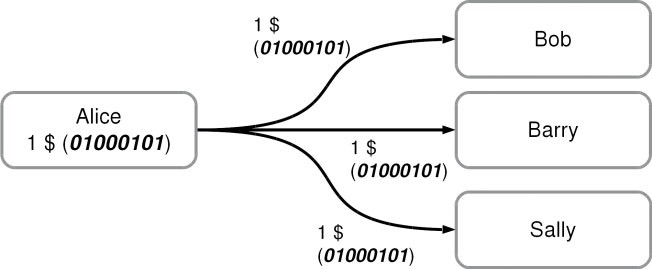
\includegraphics[width=\textwidth]{double_spending_problem.jpg}
		\caption{Double-spending problem, da "Understanding Bitcoin" \cite{understanding_bitcoin} figura 2.1}
		\label{fig:double-spending_img}
	\end{figure}

	\subsection{Database centralizzato}
		\begin{figure}[ht]
			\centering
			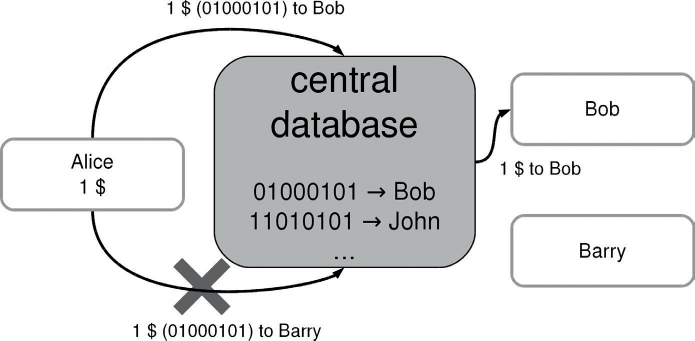
\includegraphics[width=\textwidth]{central_counterparty.png}
			\caption{Central counterparty holding a centralized database, da "Understanding Bitcoin" \cite{understanding_bitcoin} figura 2.2}
			\label{fig:central_counterparty_img}
		\end{figure}
		La soluzione contro il \emph{double-spending} finora adottata è stata l'affidamento delle transazioni economiche digitali ad un ente esterno fidato (e.g. i sistemi e-banking) che conoscesse le identità degli utenti e potesse verificarne l'effettiva disponibilità economica. È il database centrale che traccia la storia delle transazioni effettuate da ogni utente e prima di autorizzare la successiva verifica che non ci siano incongruenze. \\
		Affidarsi ad un sistema centralizzato risolve il problema, ma porta con sé una serie di criticità. \\
		Prima di tutto la necessità di \emph{trust}, fiducia, nei confronti dell'intermediario centrale: esso infatti ha libero accesso ai dati degli utenti e alla loro storia transazionale, si occupa dell'affidabilità dell'intero sistema, può autorizzare o negare transazioni e bloccare interi utenti. Si tratta di un nodo cruciale per la sicurezza del sistema, un attacco riuscito nei suoi confronti comporterebbe conseguenze disastrose. Inoltre, il database rappresenta un \emph{single point of failure}: abbattere il nodo centrale significa abbattere l'intera rete.

	\subsection{Sistemi distribuiti}
		Un'alternativa ad un sistema controllato da un intermediario centrale è rappresentata da un sistema distribuito decentralizzato. In un sistema distribuito due o più nodi collaborano per svolgere un compito prefissato in maniera trasparente all'utente, che si interfaccia con un'unica piattaforma logica. Emerge la necessità di coordinare i diversi attori: i nodi possono essere onesti e funzionare in modo corretto oppure difettosi, mal funzionanti o maliziosi. Anche se qualche nodo si rivelasse difettoso o la connessione venisse a mancare, un buon sistema distribuito dovrebbe assorbire l'imprevisto e continuare a lavorare senza problemi. La complessità di progettazione di sistemi di questo tipo non è indifferente, è stata area di ricerca fertile per molti anni e lo è tuttora. Un risultato importante è il teorema CAP, che dimostra come non possano coesistere tutte le caratteristiche desiderate in uno stesso sistema.

		\subsubsection{Teorema CAP}\label{sec:teorema_CAP}
			Altrimenti noto come Teorema di Brewer, proposto da Eric Brewer nel 1998 e dimostrato poi da Seth Gilbert e Nancy Lynch nel 2002 \cite{CAP}, il teorema CAP afferma che un qualsiasi sistema distribuito non può garantire simultaneamente le tre seguenti proprietà:
			\begin{itemize}
				\item \textbf{Coerenza (Consistency)} è la proprietà che assicura che tutti i nodi del sistema posseggono la stessa copia aggiornata dei dati;
				\item \textbf{Disponibilità (Availability)} indica che il sistema è attivo, accessibile e pronto a ricevere input e a fornire output corretti nei tempi previsti;
				\item \textbf{Tolleranza di partizione (Partition tolerance)} assicura che anche nel caso un gruppo di nodi crollasse per qualche motivo, il sistema continuerebbe ad operare correttamente.
			\end{itemize}

		\subsubsection{Problema dei Generali Bizantini}
			Si tratta di un quesito posto da Leslie Lamport (con Marshall Pease e Robert Shostak) nel 1982 \cite{BGP}, dove un gruppo di generali a capo di diverse sezioni dell'esercito bizantino sta pianificando di attaccare una città. L'unico modo a loro disposizione per comunicare è mediante messaggeri, e hanno bisogno di concordare il momento dell'attacco per vincere. Potrebbero esserci traditori tra di loro, i quali comunicherebbero messaggi discordanti per minare la riuscita dell'operazione: è quindi necessario stabilire un sistema affidabile per raggiungere il consenso sulle tempistiche di attacco. È facile l'analogia con un sistema informatico distribuito in cui i generali siano rappresentati dai nodi e i messaggeri come un'infrastruttura di rete. Una soluzione praticabile del problema dei generali bizantini in un sistema sincrono è stata proposta da Miguel Castro e Barbara Liskov in \emph{Practical Byzantine Fault Tolerance} \cite{PBFT}, mentre Bitcoin è la prima implementazione pratica con la sua soluzione basata sulla Proof-of-Work.

		\subsubsection{Algoritmi di consenso}
			La ricerca sui modi per raggiungere il consenso tra nodi di un sistema distribuito si è sviluppata molto nel periodo successivo all'introduzione di Bitcoin, pertanto sarebbe quantomeno ottimistico fornire un elenco di metodi che volesse essere esaustivo. È possibile tuttavia individuare due categorie principali di algoritmi:
			\begin{itemize}
				\item \textbf{Basati sulla fault-tolerance Bizantina}, si affidano ad un insieme di nodi che si scambiano messaggi firmati. Non richiedono impiego di risorse intensivo, sono affidabili fintanto che $N > 3F$ dove N è il numero di nodi e F è il numero di nodi malevoli;
				\item \textbf{Basati sul riconoscimento di un leader}, mettono i nodi in competizione per essere riconosciuti come leader e il nodo vincitore propone un accordo. Tipicamente richiedono un impiego di risorse considerevole come "gara" e la sicurezza delle loro applicazioni spesso si basa proprio sulla non convenienza di un tale investimento per un attaccante.
			\end{itemize}
\section{Bitcoin}


\chapter{Potenzialità e limiti}
\section{Generalizzazione}
	In seguito all'esordio di Blockchain assieme a Bitcoin sono state presentate numerose proposte per sviluppi ed implementazioni della tecnologia. Nel seguito di questa sezione si presenta quello che vuole essere uno schema delle caratteristiche salienti di un sistema basato su Blockchain: sono riportati le principali scelte di progettazione che lo caratterizzano e alcune delle soluzioni ad oggi adottate. La ricerca è estremamente attiva a riguardo, perciò questo elenco non sarà e non vuole essere esaustivo: lo scopo è quello di chiarire a che tipologie di sistema si fa riferimento parlando genericamente di \emph{Blockchain}.
	\subsection{Definizione tecnica}
		Una buona definizione generica di Blockchain è quella proposta da Imran Bashir in \emph{Mastering Blockchain} \cite{mastering_blockchain}: essenzialmente si tratta di un registro distribuito peer-to-peer, crittograficamente sicuro, append-only, immutabile (o meglio, estremamente difficile da modificare) e aggiornabile solo previo consenso da parte dei peer. Esistono ovviamente molte altre definizioni, ciascuna con enfasi diversa sui vari aspetti di Blockchain, tuttavia l'estrema sintesi di quella di Bashir permette di concentrarsi sugli aspetti imprescindibili che la caratterizzano, lasciando alle scelte di progettazione successive il compito di determinarne i particolari.
		
	\subsection{Accesso}
		La prima grande suddivisione in macro categorie dei sistemi basati su Blockchain ne riguarda le modalità di accesso. La Blockchain può essere:
		\begin{itemize}
			\item \textbf{Pubblica} nel momento in cui il sistema è aperto al pubblico e chiunque può installarne un client, scaricare il registro e partecipare attivamente ai processi di validazione dei blocchi. Tipicamente ogni utente scarica e mantiene una copia locale del registro e tramite un sistema di consenso distribuito si raggiunge un accordo con il resto della rete sull'effettivo stato ``ufficiale" dei dati. Tipicamente si affidano ad algoritmi di consenso basati su proof-of-work o proof-of-stake. Sono anche dette \emph{permissionless ledgers}, e l'esempio più noto è Bitcoin;
			\item \textbf{Privata} nel caso l'accesso sia ristretto ad un limitato insieme di utenti o organizzazioni che abbiano deciso di condividere dei registri comuni. In questa accezione di Blockchain acquista importanza l'autenticazione degli utenti, e si ottiene una maggiore riservatezza dei dati a costo di rinunciare alla natura completamente ``\emph{trustless}" delle blockchain pubbliche. Ciò porta a differenze sostanziali nella gestione del consenso: è possibile prescindere da prove onerose come la proof-of-work, e soprattutto viene a mancare la necessità di rendere vantaggioso a ciascun peer il mantenimento del sistema.
			Il grado di chiusura di questo tipo di blockchain può variare anche molto: è possibile ad esempio permettere a ciascun utente di osservare il registro ma limitarne ad un insieme ristretto la modifica. Sono anche dette \emph{permissioned ledgers} e esempi possibili sono Ripple e i sistemi costruiti su Hyperledger.
		\end{itemize}
	
	\subsection{Consenso}
		La tipologa di consenso adottata caratterizza fortemente l'intero sistema Blockchain, ed è strettamente legata alla tipologia di accesso scelta.
		\begin{itemize}
			\item \textbf{Proof of work}: è il meccanismo di consenso adottato da Bitcoin. Richiede la soluzione ad un problema matematico computazionalmente impegnativo (e.g. \emph{Hashcash}) come prova delle risorse investite per far accettare la propria proposta dalla rete;
			\item \textbf{Proof of stake}: è il meccanismo di consenso usato da Peercoin (e si parla di adottarlo prossimamente in Ethereum \cite{casper}). Sbilancia la probabilità di far accettare una proposta di cambiamento del registro in favore dei nodi di maggiore ``importanza" all'interno della rete. In una Blockchain che rappresenti una valuta, ad esempio, l'importanza consiste nella quantità di valuta posseduta. Nella variante dei consensi \emph{deposit-based} invece si acquista importanza versando quella che è in pratica una caparra. L'idea di base è che un attaccante dovrebbe investire talmente tante risorse nell'oggetto del suo attacco da renderlo non profittevole, in quanto le ricadute sul suo investimento sarebbero troppo pesanti. Una variante è la \emph{Delegated Proof of Stake} in cui i nodi importanti delegano la validazione di ciascuna transazione tramite votazione;
			\item \textbf{Proof of elapsed time}: è un meccanismo di consenso introdotto da Intel \cite{poet} allo scopo di limitare l'enorme dispendio di energie dei sistemi proof-of-work. Utilizza hardware proprietario certificato per garantire l'affidabilità di un timer, ottenendo di fatto lo stesso effetto dei PoW con irrisorio consumo di energia;
			\item \textbf{Reputation based}: è una variante dei sistemi proof-of-stake dal nome autoesplicativo. Il leader viene eletto sulla base della reputazione che si è costruito nel tempo all'interno della rete, che può basarsi su lavoro effettuato o su espressione degli altri nodi;
			\item \textbf{Federated (Byzantine) agreement}: è un sistema non-trustless, e pertanto adatto a blockchain di tipo permissioned. I nodi tengono traccia di un gruppo di peer pubblicamente riconosciuti come affidabili e propaga solo le transazioni validate dalla maggioranza dei nodi affidabili. È implementato nello Stellar Consensus Protocol \cite{stellar_protocol}; 
			\item \textbf{Practical Byzantine Fault Tolerance}: è la soluzione originale al problema dei generali bizantini proposta da Castro e Liskov nel 1999 \cite{PBFT}.
		\end{itemize}

	\subsection{Struttura}
		La scelta è in questo caso tra:
		\begin{itemize}
			\item Tokenized blockchain;
			\item Tokenless blockchain.
		\end{itemize}
		Blockchain è nata come supporto ad un sistema di scambio di token, e le applicazioni al momento più diffuse rispecchiano questo legame nei confronti di un'unità minima di informazione trasferibile. Soprattutto nel caso di blockchain permissioned, però, è possibile prescindere dal concetto di token, condividendo informazioni analogamente a quello che si può fare mediante un database tradizionale. Hyperledger permette di implementare sistemi di questo tipo, basati su un database condiviso (lo \emph{state}) in cui ogni modifica è registrata in una blockchain che funge da "log certificato".
	
	\subsection{Indipendenza}
		Un ultima distinzione degna di nota è quella tra blockchain stand-alone e sidechain \cite{sidechain}. Finora, le implementazioni di sidechain riguardano esclusivamente le tokenized blockchain. Una sidechain si appoggia ad una stand-alone e permette i trasferimenti di token dall'una all'altra. Si appoggia su varianti di proof-of-stake in cui è necessario impegnare dei coin di una catena per generarne nell'altra. I trasferimenti possono essere unidirezionali o bidirezionali. L'interesse sulle sidechain è estremamente alto poiché queste abilitano la creazione di monete che si appoggiano a criptovalute diffuse come Bitcoin e ne vanno a colmare delle lacune. Interessante a proposito il punto di vista di Ferdinando Ametrano sull'uso di sidechain per ottenere la stabilità dei prezzi con una criptovaluta, riportata nel suo paper del 2014 ``\emph{Hayek Money: the Cryptocurrency Price Stability Solution}" \cite{hayek_money}.

	\subsection{Teorema CAP e Blockchain}
		Può sembrare che le varie implementazioni di Blockchain illustrate violino il \href{sec:teorema_CAP}{teorema CAP} presentato in \ref{sec:teorema_CAP}. Ciò è inesatto: in particolare Blockchain persegue disponibilità e tolleranza di partizione in maniera istantanea, mentre la coerenza è sacrificata e ottenuta solo attraverso un lasso di tempo. Si parla in questo caso di \emph{coerenza eventuale}, ed è il motivo per cui il protocollo Bitcoin è stato di fatto artificialmente rallentato mediante un problema a difficoltà dinamica, che assicurasse un impegno per la proof-of-work di circa 10 minuti. Un qualsiasi sistema Blockchain può dirsi coerente solo facendo riferimento a transazioni con una certa ``età", che siano state accettate e validate col tempo dai vari peer.

\section{Benefici e limitazioni}
	\emph{Spunto di riflessione: blockchain innovazione sia in ambito economico che in ambito informatico: rivoluziona nel primo caso, innova nel secondo. \\
	\href{https://www.linkedin.com/pulse/ending-bitcoin-vs-blockchain-debate-gideon-greenspan}{LINK: Ending the bitcoin vs blockchain debate}}
	
	Nella gran quantità di materiale prodotto su Blockchain dalla sua presentazione ad oggi si contrappongono le posizioni di chi la considera la base della ``quarta rivoluzione industriale" \cite{4industrialrevo}, o il quinto ``disruptive computing paradigm" \cite{blockchain_swan}, a chi ne critica fortemente l'efficacia sostenendo che sia applicabile unicamente ai sistemi di cripto valute \cite{what_is_it_good_for}. \\
	L'analisi della questione è complicata dall'intrinseca interdisciplinarità dell'argomento. Ferdinando Ametrano parla di Bitcoin \cite{Ametrano_slides} come argomento all'incrocio di quattro discipline: crittografia, reti di calcolatori e trasmissione dati, teoria dei giochi e teoria economica e monetaria. Anche affrontando solamente l'aspetto tecnologico di Blockchain intesa in senso più generale, è fondamentale rendersi conto della moltitudine di sfaccettature possibili: la maggior parte dei confronti tende a semplificare e ad ignorarne alcune in favore di altre, il che conduce a conclusioni completamente diverse. Un altro punto delicato riguarda le enormi differenze tra i diversi tipi di blockchain: sebbene l'affermarsi di questa tecnologia porti indubbiamente \emph{innovazione}, non sempre si può parlare di \emph{rivoluzione} vera e propria. Per comprenderne benefici e limitazioni in maniera equilibrata, è necessario distinguere almeno le due grandi famiglie di blockchain: \emph{permissionless} e \emph{permissioned}.
	\subsection{Blockchain permissioned}
		Rappresentano l'innovazione più mite. Il controllo operato sui partecipanti al sistema permette di ridurre molti aspetti negativi della tecnologia, ma ne limita certamente il potenziale. In particolare, si può pensare a questi sistemi come ad alternative ai database tradizionali, con l'aggiunta di alcune desiderabili proprietà. Tutti i punti riportati di seguito sono applicabili anche ai sistemi permissionless e pertanto si possono considerare come caratteristiche ``generali" di Blockchain.
		\subsubsection{Vantaggi: [bozza]}
			\begin{itemize}
				\item \textbf{Semplificazione del paradigma attuale}: al momento è possibile ottenere gran parte dei vantaggi con altri sistemi, usare blockchain serve a semplificare e uniformare in un'unica architettura coerente il tutto;
				\item \textbf{Trasparenza}: ogni peer può controllare ogni transazione all'occorrenza, ideale negli scenari in cui sia necessario verificare il rispetto di norme condivise;
				\item \textbf{Condivisibilità}: la natura distribuita del sistema porta con se come diretta conseguenza la condivisione dei suoi contenuti, pur mantenendone pieno controllo sulle modifiche;
				\item \textbf{Immutabilità}: estrema difficoltà di modificare dati scritti in precendenza (impossibilità di fatto). Nel caso particolare dei sistemi permissioned, bisogna fare attenzione a non minare la sicurezza del sistema generale dando per scontata l'affidabilità degli attori;
				\item \textbf{Sicurezza}: tutte le transazioni in una blockchain sono crittograficamente protette e contribuiscono ad assicurare l'integrità del sistema;
				\item \textbf{Disponibilità del servizio}: basarsi su una rete peer-to-peer permette di garantire la disponibilità del servizio anche nel caso un certo numero di peer non fosse disponibile. Le policy di consenso influenzano anche questo punto molto pesantemente: se stabilisco che una transazione debba ricevere il consenso da tutti gli altri peer, ne basta uno non funzionante e il sistema diventa non disponibile;
			\end{itemize}
		\subsubsection{Svantaggi: [bozza]}
			\begin{itemize}
				\item \textbf{Inefficienza rispetto ai database tradizionali}
				\item \textbf{Scalabilità}
				\item \textbf{Complessità e carenza di know-how}
				\item \textbf{Tecnologia relativamente immatura}
			\end{itemize}
		
	\subsection{Blockchain pubbliche}
		Rappresentano l'aspetto rivoluzionario di Blockchain. L'idea originaria di Nakamoto ha permesso per la prima volta di generare un'entità digitale \emph{scarsa}, ovvero non arbitrariamente replicabile, senza la necessità della supervisione di un intermediario centrale. In questa tipologia si trovano i vantaggi più dirompenti, assieme ai limiti più vincolanti.
		\subsubsection{Vantaggi: [bozza]}
			\begin{itemize}
				\item \textbf{No single point of failure}
				\item \textbf{Non censurabilità o revocabilità del servizio}
				\item \textbf{Velocità di validazione}: prescindere da intermediari può portare ad un'accorciamento dei tempi necessari allo svolgimento di operazioni come quelle finanziarie;
				\item \textbf{Risparmio sulle transazioni};
			\end{itemize}
		\subsubsection{Svantaggi: [bozza]}
			\begin{itemize}
				\item \textbf{Scalabilità}: situazione estremamente più drastica di quella dei sistemi permissioned; 
				\item \textbf{Adattabilità}
				\item \textbf{Regolamentazione}
				\item \textbf{Privacy}
				\item \textbf{Impossibilità di interventi correttivi}
			\end{itemize}

\chapter{Proposta di use case}
Alla luce di quanto scritto finora, una possibile applicazione della tecnologia si può individuare nell'e-voting. Nei sistemi di voto attualmente in uso, la correttezza del voto e l’anonimato del votante sono totalmente affidati al controllo di un ente o di un sistema centrale in cui si ha fiducia come può essere lo stato o l'organo che indice la votazione. Questo vincola gli eleggibili e gli elettori ad una mancanza di trasparenza finora ritenuta inevitabile, e il sistema elettorale a dover investire risorse considerevoli nel gestire la votazione a partire da quando viene indetta fino al termine degli scrutini. L’avvento della tecnologia Blockchain permette un cambio di paradigma in favore di sistemi decentralizzati e trasparenti in cui non sia necessario riporre fiducia nell’operato di alcuno degli agenti coinvolti. Si propone quindi un modello che permetta di applicare queste caratteristiche desiderabili ad una votazione elettronica.

\section{Tecnologie e algoritmi utilizzati}
	\subsection{Hyperledger Fabric v.1.0} \label{sec:Hyperledger}
		Hyperledger è un progetto collaborativo della Linux Foundation che mira a creare un framework open source per lo sviluppo di sistemi Blockchain in ambito aziendale. Fabric è uno dei sottoprogetti che fanno parte di Hyperledger, in particolare rappresenta il principale contributo di IBM alla causa. Nella visione di Hyperledger Fabric un sistema Blockchain aziendale deve essere basato su di un'architettura modulare in cui i diversi elementi, come algoritmi di consenso, sistema di verifica delle identità, protocolli di cifratura o tipo di database ausiliari, siano intercambiabili e sostituibili liberamente. Permette anche lo sviluppo di smart contract, qui chiamati chaincode, attraverso l'uso di un qualsiasi linguaggio di programmazione: caratteristica che lo rende estremamente più flessibile del limitato set di istruzioni previsto da Bitcoin o dal linguaggio dedicato sviluppato da Ethereum. Per fare ciò l'esecuzione dei chaincode è isolata in un container dedicato, creato attraverso Docker, contenente un sistema operativo sicuro, il linguaggio del chaincode e gli SDK che permettono di interfacciarsi con il sistema. Fabric è un sistema permissioned, tutti i partecipanti sono tenuti ad autenticarsi attraverso un servizio dedicato (anche questo intercambiabile) per avere accesso alla rete. 
		\subsubsection{Componenti di Fabric}
			\begin{itemize}
				\item \textbf{Client}: sono gli enti partecipanti alla rete che invocano un chaincode o propongono una transazione. Rappresentano gli utenti finali, non mantengono una copia della blockchain ma devono connettersi con un peer per interagire con il sistema;
				\item \textbf{Peer}: sono gli enti che effettuano le transazioni e mantengono il database condiviso e la blockchain. I peer sono coordinati dall'orderer secondo delle policy specificate a priori;
				\item \textbf{Orderer}: è l'ente (eventualmente distribuito) che sovrintende alla comunicazione tra i nodi della rete. Fornisce garanzie di consegna dei messaggi immessi nella rete, tra cui le proposte di transazione da parte dei peer. È il responsabile del consenso all'interno del sistema distribuito;
				\item \textbf{Membership services}: sono l'astrazione di tutti i meccanismi crittografici e i protocolli che lavorano alla validazione dei certificati e al riconoscimento degli utenti; 
				\item \textbf{Organizzazioni}: rappresentano ciascuna entità distinta che possiede un certificato univoco per la rete. I nodi come i peer o i client devono essere legati ad un'organizzazione per poter essere riconosciuti e autenticati;
				\item \textbf{Channel}: è l'overlay della blockchain privata di Hyperledger. Ciascun canale ha un registro specifico, condiviso tra i peer registrati al canale, e ciascun ente coinvolto nella transazione deve essere autenticato ad uno specifico channel affinché questa abbia luogo;
				\item \textbf{State}: abbreviazione per "State Database", è il database in cui è salvato lo stato attuale del sistema per effettuare query sul registro in maniera efficiente. È modellato come un database chiave/valore con versionamento. Può essere completamente ricostruito dalla storia delle transazioni salvata in blockchain, il che ne garantisce il controllo sull'affidabilità;
				\item \textbf{Chaincode}: è il nome dato ai programmi salvati nella blockchain di Hyperledger. Sono invocati dalle transazioni, e possono inizializzare componenti nello state o modificarli. La loro esecuzione avviene in un container Docker isolato per garantirne la riservatezza. Incapsula la componente di business logic del sistema, ha corrispondenza diretta con quelli che in altri sistemi basati su Blockchain vengono chiamati \emph{smart contract}.
				\item \textbf{Transazioni}: sono la rappresentazione di ogni azione effettuata sul registro. Possono essere \emph{deploy transactions} che creano nuovo chaincode e lo ``installano" in un canale oppure \emph{invoke transactions} che invocano una funzione presente in un chaincode installato per effettuare letture o modifiche al ledger. Ciascuna transazione deve essere approvata e gestita dall'orderer, e viene registrata nella blockchain per la futura tracciabilità.
			\end{itemize}
		
	\subsection{Ring signature}
		Una ring signature, o firma ad anello, è un tipo di firma digitale legata ad un gruppo di utenti ciascuno in possesso di una chiave. Questo tipo di firma permette di verificare che l'autore appartiene a quel dato gruppo di utenti rendendo però computazionalmente infattibile determinare quale specifico utente esso sia. Riporto di seguito (tradotta) una possibile definizione formale \cite{ring_signature}: \\
		Si supponga che un gruppo di entità possieda le coppie di chiavi pubbliche/private $(P_1, S_1), (P_2, S_2), ..., (P_n, S_n)$. Il soggetto \emph{i} può apporre una ring signature $\sigma$ sul messaggio \emph{m} avendo in input $(m, S_i, P_1, ..., P_n)$. Chiunque può verificare la validità della firma dati $\sigma, m$ e le chiavi pubbliche coinvolte $P_1, ..., P_n$.
		\begin{figure}[ht]
			\centering
			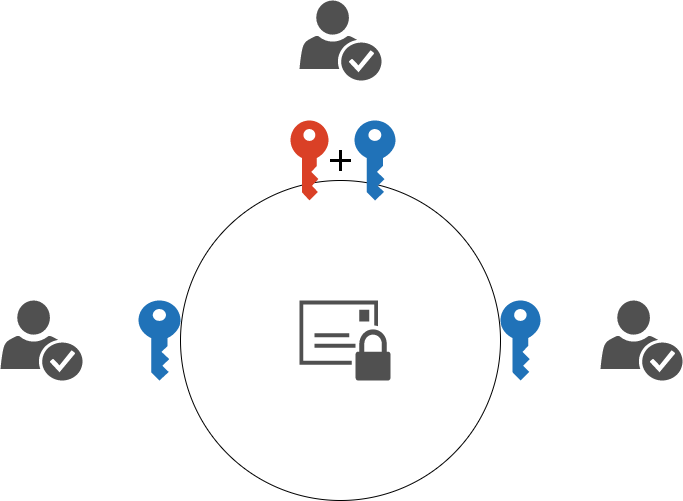
\includegraphics[width=0.6\textwidth]{ring_signature.png}
			\caption{Ring signature}
			\label{fig:ring_signature}
		\end{figure}


\section{Architettura}
	Il sistema si articola in due blockchain separate, la blockchain di firma e la blockchain di voto (da ora rispettivamente Signature chain o SC e Vote chain o VC). Le due chain sono isolate, per garantire la non collegabilità del voto al votante in fase di scrutinio.
	Le due chain hanno scopi diversi: SC assicura che il voto avvenga in maniera controllata e abilita al voto il client, inoltre contiene le informazioni per dividere in raggruppamenti i votanti similmente a quanto avviene con le sezioni elettorali; VC raccoglie i voti e li registra per effettuare poi il conteggio, ma deve garantire l’anonimato del votante.
	
	\subsection{Preparazione}
		Viene indetta una votazione. Si prevede che l'architettura sia già predisposta, in particolare devono essere noti ed affidabili, completi di chiavi pubbliche:
		\begin{itemize}
			\item L'elenco dei votanti;
			\item L'elenco dei peer;
			\item L'elenco degli indirizzi dei candidati per la Vote chain;
			\item L'elenco dei programmi client verificati.
		\end{itemize}
		\subsubsection{Inizializzazione della Signature chain}
			La SC viene predisposta con il chaincode che permette al client di interrogare la chain per conoscere le chiavi pubbliche dei votanti inseriti nello stesso raggruppamento, registrando contemporaneamente la propria firma. I dati sui raggruppamenti dei votanti sono inseriti nella SC. Questa dovrà essere accessibile solamente ai peer deputati al controllo della votazione, a causa della riservatezza delle informazioni sui raggruppamenti.
		\subsubsection{Inizializzazione della Vote chain}
			La VC contiene inizialmente delle transazioni che registrano l'associazione di ogni indirizzo numerico ad un nome intelligibile del candidato corrispondente, i saldi dei voti dei candidati inizializzati a 0 e il chaincode necessario al client per incrementare di 1 il saldo del candidato scelto. Un altro chaincode utile è quello che permette ai peer di ricevere il conteggio finale e quindi l'esito della votazione, così come il chaincode che permette ad un servizio web di interrogare la blockchain e rendere pubblici i dati in essa contenuti per permettere al votante la verifica del voto espresso.
	
	\subsection{Workflow di una votazione}
		\begin{figure}[ht]
			\centering
			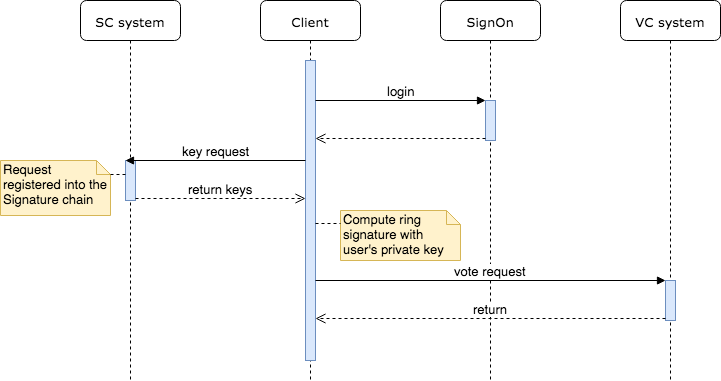
\includegraphics[width=\textwidth]{voting_workflow.png}
			\caption{Workflow della votazione}
			\label{fig:voting_workflow}
		\end{figure}
		Il diagramma in \hyperref[fig:voting_workflow]{figura \ref*{fig:voting_workflow}} illustra il workflow tipico di una votazione.
		\subsubsection{Signature chain: Firma del registro votanti}
			Il client autentica l'utente attraverso un \hyperref[subsec:personalita_voto]{sign-on affidabile}. I controlli di accesso possono essere rinforzati o meno da \hyperref[subsec:liberta_voto]{altri passaggi} affidati a sistemi di intelligenza artificiale o al controllo di un operatore. A utente autenticato, il client invoca il chaincode di query su SC ed ottiene l'elenco delle chiavi pubbliche del suo raggruppamento. Questa richiesta viene registrata in blockchain, per assicurarsi che lo stesso utente non possa ripetere la procedura di voto due volte.
			
		\subsubsection{Vote chain: In cabina elettorale}
			Il client si trova ora in possesso delle chiavi pubbliche della sua sezione. In locale permette al votante di esprimere la propria preferenza di voto e richiede la transazione corrispondente nella VC firmandola con la ring signature del proprio raggruppamento.
			La votazione è ora conclusa.
		
		\subsubsection{Scrutinio e verifica}
			Le operazioni di scrutinio e verifica possono ora essere completamente automatizzate, facendo riferimento ad una base di dati sicura e virtualmente inalterabile come la blockchain.

\section{Analisi}
	In questa sezione si analizzano le scelte architetturali fatte argomentandole, concludendo con delle possibilità di miglioramento che si potranno presentare con l'avanzamento dello scenario tecnologico attuale.
	
	\subsection{Qualità del voto}
		Il voto è definito dall'art. 48 \cite{art48} della Costituzione Italiana come "personale ed eguale, libero e segreto".
		\subsubsection{Personalità}\label{subsec:personalita_voto}
			La personalità del voto, intesa come la necessità di esercitarlo di persona e non tramite terzi, è delegata in questa proposta al servizio di sign-on. Al momento attuale, è possibile fare affidamento su diversi sistemi di autenticazione: per il corretto funzionamento del sistema è previsto che ogni utente abbia una coppia di chiavi pubblica e privata distribuita precedentemente, sotto verifica di un operatore. Ad esempio, è possibile distribuire queste chiavi contestualmente alla consegna della tessera elettorale. La natura certificata di queste chiavi le rende ideali come metodo di autenticazione ma è possibile aggiungere ulteriori controlli come una verifica tramite dati biometrici.
		
		\subsubsection{Eguaglianza}
			L'eguaglianza del voto consiste nell'avere ogni voto lo stesso valore di tutti gli altri. Si articola nell'impedire, in particolare, il voto plurimo e il voto multiplo. Nel sistema proposto, il voto plurimo è scongiurato dal codice del chaincode della Vote chain, il quale permette solo incrementi unitari al saldo dei candidati. Uno scenario di voto multiplo è invece controllato dalla Signature chain e dalla struttura del client: è infatti indispensabile che la procedura di voto sia strettamente successiva alla procedura di firma in SC, e non invocabile in maniera indipendente. In tal modo è possibile garantire che una stessa persona non reiteri l'esecuzione del chaincode di voto. Pur ammettendo il caso in cui un attaccante riesca a violare il client, questo potrà reiterare voti firmati dalla stessa ring signature: un controllo automatico può facilmente accorgersi della non coerenza del numero di votanti nel raggruppamento e il numero di voti espressi dal raggruppamento, invalidando di fatto le transazioni ma mantenendo confinato l'evento disastroso: si possono applicare le procedure invocate attualmente qualora venissero riscontrate irregolarità che compromettano la validità dei voti di una sezione elettorale.
		
		\subsubsection{Libertà}\label{subsec:liberta_voto}
			La libertà del voto viene garantita dal negare la possibilità di voto qualora il votante fosse stato costretto con mezzi illeciti a esprimere una certa preferenza. Nel sistema di voto attuale è garantita dal controllo degli operatori di seggio. Nei sistemi di voto remoto l'argomento risulta spinoso: è infatti estremamente difficile stabilire una situazione di particolare pressione dell'elettore, o l'interferenza di esterni. Nel caso di voto elettronico, forzare il client ufficiale a poter essere installato solo su dispositivi muniti di telecamera frontale potrebbe risolvere il problema. Il controllo può essere svolto da appositi addetti eventualmente aiutati da un'intelligenza artificiale simile a quella utilizzata da Unilever \cite{ai_unilever} per i colloqui di lavoro. Questo non scongiura ogni possibile manipolazione, ma va evidenziato che il controllo sul sistema proposto non lo rende meno sicuro del sistema già in essere: permette anzi un livello di garanzia estremamente più alto di quello dei sistemi di voto per corrispondenza, già accettati in Italia in caso di votanti dall'estero e adottato in maniera diffusa in Svizzera.
		
		\subsubsection{Segretezza}
			La segretezza del voto nel sistema proposto ha come fulcro la completa separazione delle due blockchain. Affidando al client il compito di mantenere la continuità dell'operazione di voto, l'accoppiamento tra votante e voto espresso non può essere ricostruito con certezza in alcun modo. L'unica informazione che può trapelare riguarda il momento in cui viene registrata la votazione nelle due chain, tuttavia questa informazione è molto meno affidabile di quanto possa sembrare a causa della \href{sec:teorema_CAP}{consistenza eventuale} della blockchain. Sebbene qualche informazione trapeli, l'elevato numero di transazioni contemporanee previsto e l'incertezza nel determinare l'esatto momento di voto rende di fatto inservibili queste informazioni.
	
	
	\subsection{Necessità dei raggruppamenti}
		La suddivisione in sezioni elettorali è assolutamente necessaria nel sistema di voto attualmente adottato a causa di problemi logistici: è impensabile infatti raggruppare tutte le schede e svolgere un'unica operazione di scrutinio, soprattutto considerando il livello di sorveglianza che sarebbe richiesto in ogni momento dell'operazione. In un sistema automatico come quello proposto, esente da queste problematiche, sono stati introdotti raggruppamenti di elettori per differenti ragioni. In primo luogo, la complessità computazionale degli algoritmi più noti e affermati per la ring signature è lineare: questo preclude l'uso significativo di questa tecnologia (centrale nel modello proposto) per insiemi di chiavi sufficientemente grandi. In secondo luogo, nel caso un attacco permettesse di replicare lo stesso voto più volte la divisione in raggruppamenti permette di contenere i danni al solo raggruppamento interessato.
		È da sottolineare come, nel caso di un sistema elettronico, l'indipendenza dai problemi logistici dei sistemi tradizionali permetta di variare di volta in volta la composizione dei raggruppamenti, rendendo inutile qualsiasi informazione trapelata dalle votazioni precedenti. Questa è una condizione certamente più sicura di quella attuale, dove una semplice osservazione sul posto permette di identificare gli appartenenti a ciascuna sezione e far trapelare quindi informazioni (per quanto parziali) sulle preferenze di voto espresse: essendo i risultati delle votazioni per seggio pubblici, il trapelare di qualsiasi informazione sulla composizione del seggio è da considerarsi quantomeno indesiderato.
	
	\subsection{Prevedibili miglioramenti futuri al sistema}
		Al momento passaggi critici come l'autenticazione utente e il passaggio dalla SC alla VC devono essere svolti off-chain, ma future scoperte potrebbero aprire la strada verso implementazioni più complete.
		Portare l'autenticazione utente su Blockchain è un progetto che si lega con la creazione di un sistema di identità digitale decentralizzata. Immaginando un futuro (ad ora remoto) in cui siano disponibili documenti affidabili on-chain attraverso qualche tecnologia, l'autenticazione utente potrebbe svolgersi in questo modo guadagnando le caratteristiche di decentralità e sicurezza proprie della Blockchain. \\
		Più vicino alla situazione attuale è un meccanismo che permetta di abilitare alla votazione su VC direttamente da SC, senza rinunciare all'anonimato del votante. Al momento, ogni chaincode di Hyperledger è eseguito in un ambiente completamente isolato per ragioni di sicurezza. Sono già previste successive implementazioni che permettano a diversi chaincode di interagire tra di loro. Questo aprirebbe ad una modifica del sistema di voto proposto: sarebbe possibile implementare su VC un sistema di token: questi token sarebbero generati quando viene indetta la votazione in base al numero di aventi diritto al voto, e versati dai chaincode verso dei ``portafogli" temporanei da loro generati casualmente. Questi sarebbero poi passati al client già cifrati in maniera da mantenere chiunque, eccetto il software del chaincode, all'oscuro dell'accoppiamento votante-portafoglio. In questo modo sarebbe possibile prescindere dai raggruppamenti affidando la sicurezza del sistema unicamente alla solidità della Blockchain. L'aspetto negativo è che si perderebbe la capacità dei raggruppamenti di confinare un eventuale attaccante.

\chapter{Scenario attuale e sfide future}
\section*{DISCLAIMER} \emph{Questa sezione è un cantiere aperto. NON è definitiva in nessuna sua parte, NON nei contenuti, NON nella struttura, NON nel tono generale del discorso. Si tratta di una serie di appunti che sto prendendo e che saranno la base su cui scriverò poi la versione definitiva, li inserisco per mantenerne traccia e per avere ben chiara la direzione che sta intraprendendo il discorso.}

In questo capitolo si vuole presentare il quadro attuale della situazione attorno ai sistemi blockchain. Nuove tecnologie sono sviluppate continuamente, perciò dopo una breve panoramica sui progetti più interessanti già in stadio avanzato di sviluppo si illustreranno le sfide e gli ambiti di ricerca più ferventi, fino ad arrivare ad elencare alcune delle applicazioni che potrebbero conseguire dai risultati di tali ricerche.

\section{Innovazioni vicine}
    Al momento si assiste ad una crescita rapidissima di Bitcoin, tale da portare l'argomento al di fuori degli ambiti specialistici e farlo diventare un vero e proprio fenomeno di massa.
    \begin{figure}[ht]
        \centering
        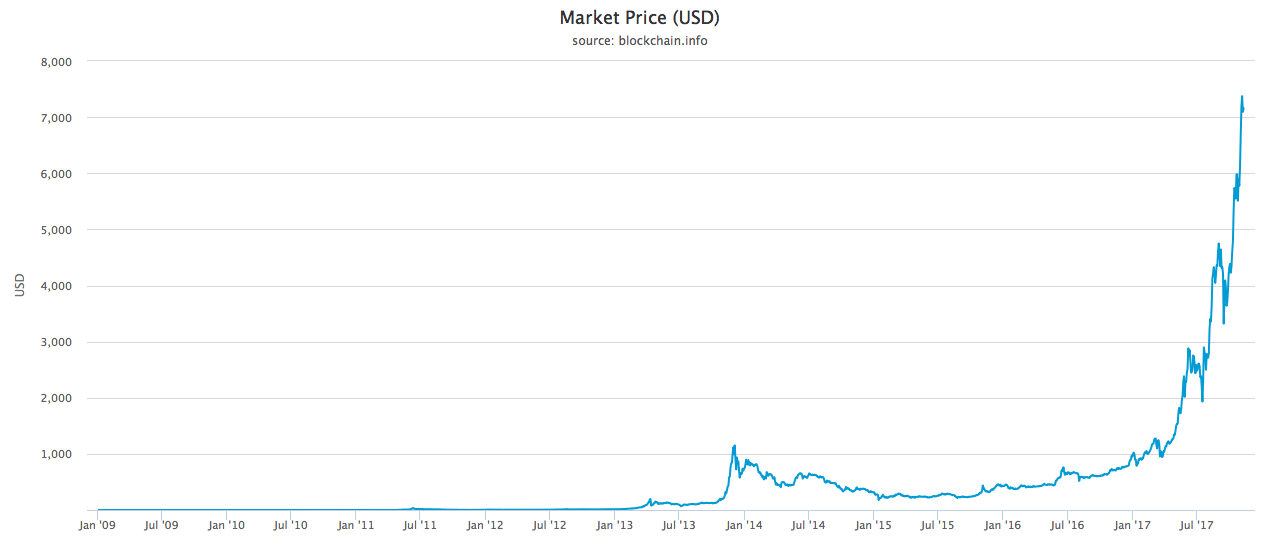
\includegraphics[width=\textwidth]{bitcoin-price.png}
        \caption{Valore di mercato di bitcoin}
        \label{fig:bitcoin_price}
    \end{figure}
    Dietro a Bitcoin si sta sviluppando un'enorme quantità di applicazioni e sperimentazioni che riguardano Blockchain, alcune delle quali hanno raggiunto ormai una certa stabilità. Molte di queste riguardano l'ambito economico e prendono il nome di \emph{criptomonete}, altre invece si basano sulla blockchain per costruire sistemi più complessi.
    \subsection{Criptomonete}
        \begin{itemize}
            \item \textbf{Ripple}: è il più famoso sistema di scambio di valuta basato su blockchain permissioned, adottato tra gli altri da MUFG, RBC, Santander, Unicredit, BBVA \url(https://ripple.com/);
            \item \textbf{Litecoin}: è una criptomoneta molto simile a Bitcoin da cui differisce per alcune caratteristiche chiave, su tutte il tempo necessario all'elaborazione di un blocco (2 minuti e mezzo contro i 10 minuti di Bitcoin) e il sistema di consenso. Litecoin infatti usa \emph{scrypt} per la sua proof-of-work, una funzione gravosa sulla memoria piuttosto che sul processore che punta a evita il predominio delle server farm con hardware dedicato che controllano le operazioni di mining di Bitcoin;
            \item \textbf{Peercoin}: è una criptomoneta alternativa che adotta un algoritmo di consenso ibrido tra proof-of-work e proof-of-stake, allo scopo di portare un'alternativa solida all'enorme consumo energetico di Bitcoin;
            \item \textbf{Monero}: fork di Bitcoin che utilizza CryptoNote, un protocollo basato sulla Ring Signature orientato a rafforzare l'anonimato nella blockchain;
            \item \textbf{ZCash e ZCoin}: come Monero si pongono l'obiettivo di garantire la privacy in un sistema Blockchain, usano algoritmi di tipo zero-knowledge sebbene con piccole differenze tra di loro \cite{zcoin_vs_zcash};
        \end{itemize}
        Un'altra applicazione interessante a livello economico è quella legata all'uso di criptomonete per il crowd-funding. Questa trova una semplice implementazione direttamente in Bitcoin attraverso l'uso di quello che si chiama \emph{assurance contract}. Si tratta di una transazione con un singolo output rappresentante l'obiettivo del finanziamento, a cui si unisce poi ciascun volontario partecipante tramite hash di tipo \emph{SIGHASH\_ALL} e \emph{SIGHASH\_ANYONECANPAY}, che permettono di modificare gli input di transazione ma non gli output (si rimanda alla documentazione ufficiale per approfondimento). La transazione può essere registrata in blockchain, e quindi essere effettiva, solo quando il valore di output è coperto da corrispondente valore in input, ovvero al raggiungimento dell'obiettivo della campagna di crowd-funding.
     
    \subsection{Non-Criptomonete}
        \begin{itemize}
            \item \textbf{Ethereum}: \emph{DA ESPANDERE E PROMUOVERE A SEZIONE ASSIEME AD HYPERLEDGER} si tratta del principale sistema basato su Blockchain dopo Bitcoin. Il suo scopo è quello di permettere la creazione di applicazioni decentralizzate, che vengono eseguite come smart contract distribuiti tra i peer che partecipano alla rete. È il primo sistema blockchain ad aver introdotto un linguaggio Turing-completo (\emph{Solidity}) e il concetto di macchina virtuale su blockchain, nel 2013. Si basa su una propria moneta virtuale che viene utilizzata per ``alimentare" le applicazioni distribuite (in ambito Ethereum si parla di \emph{gas}, abbreviazione di \emph{gasoline}). Questa si chiama \emph{Ether}, e al momento si trova saldamente al secondo posto come market cap dietro a Bitcoin;
            \item \textbf{OpenTimestamps}: servizio che mira a diventare uno standard per il timestamping via blockchain. Concatena hash crittografici dei dati di cui gli utenti richiedono il timestamping e ne registra il risultato in una transazione bitcoin, rendendolo quindi pubblico e immutabile;
            \item \textbf{Namecoin}: servizio basato su blockchain che si propone di potenziare decentralizzazione, sicurezza, resistenza alla censura, privacy e velocità di componenti alcune dell'infrastruttura di Internet come i DNS;
            \item \textbf{Everledger}: una nicchia promettente riguarda i sistemi ad-hoc con utilizzo ben preciso. Ne è un esempio Everledger, che si propone di tracciare e gestire storia e possesso di beni di lusso come i diamanti; \emph{Filament} per reti wireless sicure in IoT;
            \item \textbf{Filament}: la natura distribuita di Blockchain la rende ideale per implementazione di applicazioni IoT che richiedano un adeguato livello di sicurezza. Lavora in questo ambito Filament, startup nata recentemente, nel 2017, che si pone come obiettivo la gestione di reti wireless sicure in ambito IoT;
            \item \textbf{Blockchain a livello enterprise}: per la creazione di applicazioni aziendali basate su Blockchain è necessario appoggiarsi ad opportuni framework. Questi devono rispettare requisiti imprescindibili per l'ambito business, tra cui fornire opportuna documentazione, supporto tecnico e rendere agevoli le operazioni di testing, integrazione, controlli di sicurezza. Esempi di piattaforme simili in sviluppo sono Hyperledger, Bloq, Chain, sebbene ciascuno di questi soffra al momento di poca stabilità dovuta alla loro ancora recente nascita;
            \item \textbf{Hawk}: è un sistema di smart contract che affronta il problema della poca privacy nelle transazioni delle blockchain più diffuse. Hawk fornisce uno strumento per la generazione di un ``protocollo crittografico efficiente in cui le controparti del contratto interagiscono con la blockchain usando primitive crittografiche come gli algoritmi \emph{zero-knowledge proof}." \cite{hawk};
        \end{itemize}

\section{Sfide e ambiti di ricerca}
    \subsection{Efficienza e scalabilità}
        \begin{itemize}
            \item Algoritmi di consenso
            \item Problemi crittografici nuovi
        \end{itemize}
        Il problema della scalabilità dei sistemi blockchain è molto dipendente dall'algoritmo di consenso implementato. Quelli ad oggi adottati su larga scala sono basati su proof-of-work, che paradossalmente basa la sua sicurezza sulla sua assoluta inefficienza. Inoltre, la storia di Bitcoin mostra come sia inefficace nel mantenere equilibrata la competizione tra i miner, portando un accentramento delle capacità di gestione della rete nelle mani di server farm dedicate. Ethereum migliora questo aspetto attraverso un algoritmo simile, ma in cui ha meno vantaggi investire in hardware dedicato. Tuttavia la ricerca ad un algoritmo che permetta l'effettiva ``democratizzazione'' del mining è ancora apertissima, accompagnata da quella su problemi crittografici meno parallelizzabili su cui basare ulteriori varianti degli algoritmi proof-of-work.
        
    \subsection{Standardizzazione e interoperabilità}
        Blockchain non è ancora una tecnologia sufficientemente matura da permettere una piena ed agevole integrazione con i sistemi esistenti. Emettere degli standard adeguati aiuterà a migliorare l'integrazione dei sistemi blockchain tanto fra di loro quanto con l'infrastruttura circostante. \\
        Dal punto di vista applicativo lo sviluppo di framework come Hyperledger aiuta a creare una base solida e delle sottostrutture chiare per la progettazione di reti distribuite interoperanti, e maggiore sarà il numero di utenti che abbracceranno soluzioni di questo tipo minori saranno le differenze critiche tra sistema e sistema permettendo adattamenti più agevoli. D'altra parte, è necessario che tali piattaforme si sviluppino e allarghino la gamma di scenari modellabili venendo incontro alle necessità di gruppi di utenti sempre più grandi ed eterogenei. \\
        Dal punto di vista normativo invece si sono visti passi in avanti con la creazione nel 2016 del comitato tecnico ISO/TC 307 ``Blockchain and distributed ledger technologies", che sta sviluppando il primo standard ISO ufficiale sull'argomento.

    \subsection{Privacy}
        
        \subsubsection{Obfuscation}
            vedi pag 244 di Understanding Bitcoin
        \subsubsection{Algoritmi zero-knowledge}
            \begin{itemize}
                \item \textbf{Zero-Knowledge Password Proof} \\
                    \url{https://en.wikipedia.org/wiki/Zero-knowledge_password_proof}
                \item \textbf{Piattaforma Enigma} \\
                        \url{https://www.enigma.co/enigma_full.pdf}
                \item \textbf{zk-SNARK} \\
                    \url{https://z.cash/technology/zksnarks.html}
            \end{itemize}

\section{Cosa si potrà fare}
    \begin{itemize}
        \item Reti IoT sicure basate su Blockchain condivise
        \item Condivisione dati sensibili (cartelle cliniche?)
        \item Digital Identity
        \item Immigrazione e controlli doganali
        \item Cronotachigrafi
        \item Gestione DRM (digital rights management)
        \item Digital assets e smart properties
        \item Moneta basata su Bitcoin per transazioni efficaci tra privati
\end{itemize}


\chapter{Conclusioni}
\section{Valutazione retrospettiva}
	L'esperienza di stage è stata assolutamente positiva. L'argomento si è rivelato particolarmente complesso da comprendere, ma l'approccio adottato, il supporto e gli stimoli ricevuti sono stati più che adeguati e mi hanno permesso un percorso di crescita estremamente soddisfacente. La natura interdisciplinare del progetto mi ha portato ad approfondire argomenti accennati ma non particolarmente approfonditi nel corso degli studi per la laurea triennale quali tecnologie di rete, sicurezza e crittografia. Inoltre, la mancanza di testi universalmente adottati come riferimento mi ha portato a consultare una gran quantità di materiale fino ad arrivare ad affrontare direttamente le pubblicazioni scientifiche sull'argomento, cosa che si è rivelata estremamente interessante e che immagino si rivelerà molto utile in futuro. A corollario, ho trovato piacevoli spunti di riflessione anche nell'osservare più linguaggi di programmazione diversi da quelli affrontati nel corso di laurea (tra cui, ma non solo, Go e Solidity) e nel confronto tra loro e quanto già imparato finora.
	
	Sono consapevole della fortuna avuta nel poter confrontarmi con argomenti tanto attuali quanto stimolanti nel contesto di un'attività di tirocinio, ringrazio moltissimo i miei referenti interni all'azienda Enrico Notariale e Luca Brizzolari per le innumerevoli opportunità di confronto offertemi e mi auguro di poter proseguire i miei studi sull'argomento attraverso ulteriori esperienze in azienda e il corso di laurea magistrale.
	
	\subsection{Raggiungimento degli obiettivi}
		Nel piano di lavoro erano stati individuati i seguenti obiettivi:
		\begin{itemize}
			\item \textbf{Minimi:}
				\begin{itemize}
					\item \textbf{min01}: Analisi delle potenzialità della tecnologia blockchain, in particolare Hyperledger Fabric;
					\item \textbf{min02}: Installazione dell’architettura in un ambiente di sviluppo;
					\item \textbf{min03}: Creazione di un ambiente di sviluppo.
				\end{itemize}
			
			\item \textbf{Massimi}:
				\begin{itemize}
					\item \textbf{max01}: SWOT Analysis;
					\item \textbf{max02}: Predisposizione di una demo.
				\end{itemize}
			
			\item \textbf{Formativi}:
				\begin{itemize}
					\item \textbf{for01}: Acquisizione abilità nella gestione di aspetti riguardanti l’analisi di un progetto innovativo in un ambito aziendale (e.g. nuovi linguaggi, sistemi);
					\item \textbf{for02}: Interagire con un progetto Open-Source e la relativa community;
					\item \textbf{for03}: Sperimentare tecnologie interessanti per l’ingresso nel mondo del lavoro.
				\end{itemize}
		\end{itemize}
		
		Nel complesso posso dire raggiunti gli obiettivi pianificati, quasi tutti rispettando in pieno le aspettative. L'unico punto in cui è stato necessario scendere a compromessi è stata la predisposizione della demo: sebbene sia stata progettata e sia stato predisposto un accenno di implementazione, questa non può certo dirsi completa. La mutevolezza della piattaforma su cui stavamo lavorando si è resa evidente con la presenza di file nel repository non ancora documentati, e cambiamenti considerevoli da una settimana all'altra. Di conseguenza, si è ritenuto più proficuo indugiare nelle attività di analisi e confronto tra tecnologie riservando a progetti futuri l'implementazione effettiva del prototipo.
		
\section{Conclusioni e prosieguo del progetto}
	In conclusione, l'esperienza di tirocinio ha confermato quanto suggerito dagli studi di Gartner: Blockchain è una realtà tanto dirompente quanto delicata da implementare in ambito business. Soffre dei problemi di gioventù tipici di un sistema innovativo, a cui vanno ad aggiungersi criticità specifiche dovute alla sua complessità e al suo orientamento a sistema certificatore e garante, che non consente incertezze di rischio nel suo utilizzo. Nonostante ciò, promette innovazioni troppo importanti per essere ignorata. Ciò suggerisce una riflessione alle aziende più attente all'argomento: conviene approfittare di questo periodo di incubazione per studiare, sperimentare e accumulare le conoscenze necessarie per essere operativi e consapevoli nel seguire l'evoluzione tecnologica dei prossimi anni. 
	
	In accordo con i miei referenti, nel prossimo periodo continueranno i miei rapporti con Infocamere per proseguire ed integrare quanto fatto finora consolidando le conoscenze acquisite e arrivando sperabilmente ad una implementazione efficace di una o più sperimentazioni. Sono convinto che questo percorso possa portare l'azienda ad acquisire quella confidenza necessaria per perseguire i propri obiettivi di ricerca e innovazione, e possa portare a me una crescita inestimabile dal punto di vista intellettuale e professionale che spero di riuscire a ricambiare con risultati adeguati.
	
	
	
	
	
	
	
	
	
	
	
	
	
	
	
	
	
	
	
	
	
	

\appendix

\chapter{Implementazione}
\definecolor{mygreen}{rgb}{0,0.6,0}
\definecolor{mygray}{rgb}{0.5,0.5,0.5}
\definecolor{mymauve}{rgb}{0.58,0,0.82}

\lstset{
	basicstyle=\footnotesize \ttfamily,
	commentstyle=\color{mygreen},
	keywordstyle=\color{blue},
	stringstyle=\color{mymauve},
	numbers=none,
	%numberstyle=\tiny\color{lightgray},
	%numbersep=5pt,
	%frame=single,
	rulecolor=\color{mygray}, 
	breakatwhitespace=false,         % sets if automatic breaks should only happen at whitespace
	breaklines=true,                 % sets automatic line breaking
	tabsize=4
}

\definecolor{darkgray}{rgb}{.4,.4,.4}
\definecolor{purple}{rgb}{0.65, 0.12, 0.82}

%define Javascript language
\lstdefinelanguage{JavaScript}{
	keywords={typeof, new, true, false, catch, function, return, null, catch, switch, var, if, in, while, do, else, case, break},
	keywordstyle=\color{blue}\bfseries,
	ndkeywords={class, export, boolean, throw, implements, import, this},
	ndkeywordstyle=\color{darkgray}\bfseries,
	identifierstyle=\color{black},
	sensitive=false,
	comment=[l]{//},
	morecomment=[s]{/*}{*/},
	commentstyle=\color{purple}\ttfamily,
	stringstyle=\color{red}\ttfamily,
	morestring=[b]',
	morestring=[b]"
}

\lstset{
	language=JavaScript,
	extendedchars=true,
	basicstyle=\footnotesize\ttfamily,
	showstringspaces=false,
	showspaces=false,
	numbers=none,
	numberstyle=\footnotesize,
	numbersep=9pt,
	tabsize=2,
	breaklines=true,
	showtabs=false,
	captionpos=b
}

%\section{Costruzione della rete}
%	\lstinputlisting[language=bash]{chapters/code/build.sh}
	
%\section{Configurazione crypto-tool}
%	\lstinputlisting{chapters/code/crypto-config.yaml}
	
%\section{Configurazione configtxgen}
%	\lstinputlisting{chapters/code/configtx.yaml}

%\section{Compose}
%	\lstinputlisting{chapters/code/docker-compose.yml}
	
\section{Utilizzo del composer}
	\subsection{Creare una nuova struttura di rete}
		Il concetto chiave nell'utilizzo di Hyperledger Composer è la \emph{``business network definition" (BND)}, che definisce il modello dei dati, le regole di accesso e la logica delle transazioni della nostra rete. Per creare la scheletro del progetto si può usare Yeoman generator, installato in precedenza assieme al Composer:
\begin{lstlisting}
yo hyperledger-composer:businessnetwork
\end{lstlisting}
		Inseriamo ``voting-network" come nome della rete e ``eurasia.voting" come namespace.
	\subsection{Definire le caratteristiche della rete}
		La nostra rete si fonda su asset (e.g i raggruppamenti di votanti), partecipanti (e.g votanti e candidati), transazioni come quella che permette ad un utente di votare e query che consentano la consultazione agevole dei dati. Come output del comando precedente, c'è un file di modello (\emph{.cto}) che conterrà le definizioni di ciascuna classe di asset, transazioni, partecipanti ed eventi. Il contenuto di questo file sarà:
\begin{lstlisting}
/**
* My voting network
*/

namespace eurasia.voting

asset VotingGroup identified by groupId {
	o String groupId
	--> Voter[] members
}

asset Vote identified by voteSig {
	o String voteSig
	--> VotingGroup group
	--> Candidate recipient
}

participant Voter identified by voterId {
	o String voterId
	o String firstName
	o String lastName
}

participant Candidate identified by candidateId {
	o String candidateId
	o String firstName
	o String lastName
	o Integer balance
}

transaction Voting {
	o String signature
	--> VotingGroup group
	--> Candidate recipient
}
\end{lstlisting}
	\subsection{Scrivere la logica delle transazioni in JavaScript}
		Nel file di modello è stata definita una transazione \emph{Vote}, il cui scopo è quello di creare un nuovo voto ed indirizzarlo al candidato prescelto. Editiamo il file \emph{logic.js} per specificare il comportamento di questa transazione usando il linguaggio JavaScript, prestando attenzione ad utilizzare la sintassi accettata dal Transaction processor di Composer.
\begin{lstlisting}[language=JavaScript]
/**
* Vote for a candidate
* @param {eurasia.voting.Voting} voting - the vote to be processed
* @transaction
*/
function newVote(voting) {	
	// Get the factory for creating new asset instances
	var factory = getFactory();
	// Create the vote.
	var vote = factory.newResource('eurasia.voting', 'Vote', computeSig(voting.signature));
	vote.group = voting.group;
	vote.recipient = voting.recipient;
	voting.recipient.balance++;
	return getAssetRegistry('eurasia.voting.Vote')
		.then(function (assetRegistry) {
			// Update the asset in the asset registry. Again, note
			// that update() returns a promise, so so we have to return
			// the promise so that Composer waits for it to be resolved.
			return assetRegistry.add(vote)
		})
		.then(function () {
			return getParticipantRegistry('eurasia.voting.Candidate')
		})
		.then(function (participantRegistry) {
			return participantRegistry.update(voting.recipient);
		});
}

/*
* This function should represent the implementation of a linkable ring signature algorythm. In this PoC it will return a simple timestamp + an arbitrary id
*/
function computeSig(mySig){
	var sig = new Date().valueOf();
	sig += mySig;
	return sig;
}

\end{lstlisting}
	\subsection{Aggiungere il controllo agli accessi}
		Creiamo il file \emph{permissions.acl} nella cartella \emph{voting-network}, e al suo interno specifichiamo le regole per il controllo degli accessi in questo modo:
\begin{lstlisting}
/**
* Access control rules for voting-network
*/
rule Vote {
	description: "Allow all voters to vote through a transaction"
	participant: "eurasia.voting.Voter"
	operation: CREATE, UPDATE
	resource: "eurasia.voting.Vote"
	transaction: "eurasia.voting.Voting"
	action: ALLOW
}

rule SystemACL {
	description:  "System ACL to permit all access"
	participant: "ANY"
	operation: ALL
	resource: "org.hyperledger.composer.system.**"
	action: ALLOW
}

rule NetworkAdminUser {
	description: "Grant business network administrators full access to user resources"
	participant: "org.hyperledger.composer.system.NetworkAdmin"
	operation: ALL
	resource: "**"
	action: ALLOW
}

rule NetworkAdminSystem {
	description: "Grant business network administrators full access to system resources"
	participant: "org.hyperledger.composer.system.NetworkAdmin"
	operation: ALL
	resource: "org.hyperledger.composer.system.**"
	action: ALLOW
}
\end{lstlisting}

	\subsection{Generare il Business network archive}
		Terminata la definizione delle proprietà della rete è necessario impacchettarla in un file \emph{.bna} che rappresenta un archivio esportabile da cui poter poi effettuare il deploy su un sottostante sistema Fabric.
		Per fare ciò è necessario:
		\begin{itemize}
			\item Spostarsi nella cartella \emph{voting-network}
			\item Lanciare il seguente comando da terminale:
				\begin{lstlisting}
composer archive create -t dir -n .
				\end{lstlisting}
		\end{itemize}
		Al termine dell'esecuzione potremo trovare un file chiamato \emph{voting-network@0.0.1.bna} nella cartella da cui abbiamo lanciato il comando.

\bibliography{chapters/bibliografia}{}
\bibliographystyle{plain}

\end{document}